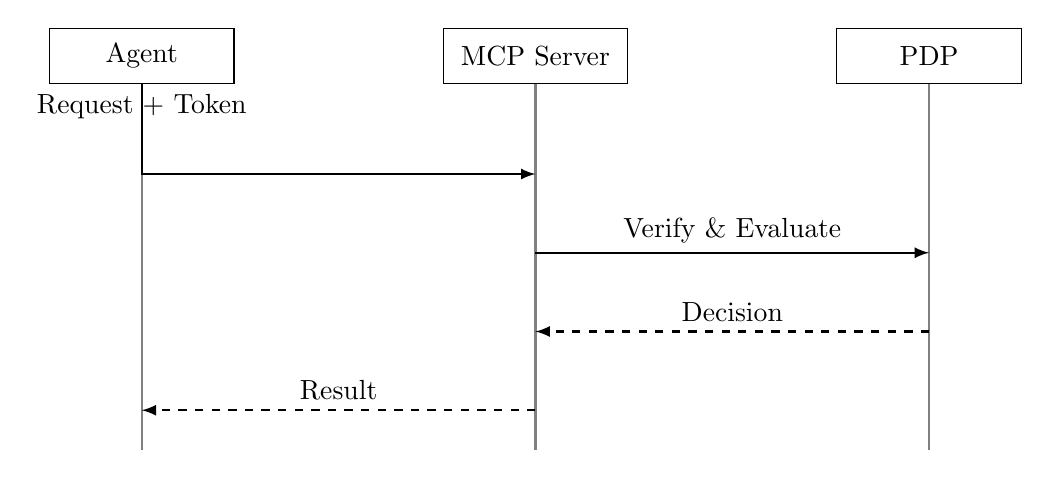
\begin{tikzpicture}[node distance=2.5cm, auto,
    participant/.style={rectangle, draw, fill=white, text centered, minimum height=2em, text width=6em},
    line/.style={draw, ->, >=latex, thick}]

    % Participants
    \node [participant] (agent) {Agent};
    \node [participant, right of=agent, node distance=5cm] (server) {MCP Server};
    \node [participant, right of=server, node distance=5cm] (pdp) {PDP};

    % Time lines
    \draw [thick, gray] (agent) -- ++(0,-5);
    \draw [thick, gray] (server) -- ++(0,-5);
    \draw [thick, gray] (pdp) -- ++(0,-5);

    % Steps
    % 1. Request
    \draw [line] (agent) -- node [above] {Request + Token} ++(0,-1.5) -- (server |- 0,-1.5);
    
    % 2. Verify & Evaluate
    \draw [line] (server |- 0,-2.5) -- node [above] {Verify \& Evaluate} (pdp |- 0,-2.5);
    
    % 3. Decision
    \draw [line, dashed] (pdp |- 0,-3.5) -- node [above] {Decision} (server |- 0,-3.5);
    
    % 4. Result
    \draw [line, dashed] (server |- 0,-4.5) -- node [above] {Result} (agent |- 0,-4.5);

\end{tikzpicture}